%% Begin slides template file
\documentclass[11pt,t,usepdftitle=false,aspectratio=169]{beamer}
%% ------------------------------------------------------------------
%% - aspectratio=43: Set paper aspect ratio to 4:3.
%% - aspectratio=169: Set paper aspect ratio to 16:9.
%% ------------------------------------------------------------------
\usepackage{graphicx}
\usetheme[nototalframenumber,logo,license]{uibk}
%% ------------------------------------------------------------------
%% - foot: Add a footer line for conference name and date.
%% - logo: Add the university logo in the footer (only if 'foot' set).
%% - bigfoot/sasquatch: Larger font size in footer.
%% - nototalslidenumber: Hide the total number of slides (only if 'foot' set)
%% - license: Add CC-BY license symbol to title slide (e.g., for conference uploads)
%%   (TODO: At the moment no other licenses are supported.)
%% - licenseall: Add CC-BY license symbol to all subsequent slides slides
%% - url: use \url{} rather than \href{} on the title page
%% ------------------------------------------------------------------

%% ------------------------------------------------------------------
%% The official corporate colors of the university are predefined and
%% can be used for e.g., highlighting something. Simply use
%% \color{uibkorange} or \begin{color}{uibkorange} ... \end{color}
%% Defined colors are:
%% - uibkblue, uibkbluel, uibkorange, uibkorangel, uibkgray, uibkgraym, uibkgrayl
%% The frametitle color can be easily adjusted e.g., to black with
%% \setbeamercolor{titlelike}{fg=black}
%% ------------------------------------------------------------------

%\setbeamercolor{verbcolor}{fg=uibkorange}
%% ------------------------------------------------------------------
%% Setting a highlight color for verbatim output such as from
%% the commands \pkg, \email, \file, \dataset
%% ------------------------------------------------------------------


%% information for the title page ('short title' is the pdf-title that is shown in viewer's titlebar)
\title[IoT Light Bulb Attack]{IoT Light Bulb Covert Channel}
\subtitle{Extended Functionality Attack on Smart Lights}
\URL{}

\author[Julia Wanker \& Bennett Piater]{Julia Wanker, Bennett Piater}
%('short author' is the pdf-metadata Author)
%% If multiple authors are required and the font size is too large you
%% can overrule the font size of author and url by calling:
%\setbeamerfont{author}{size*={10pt}{10pt},series=\mdseries}
%\setbeamerfont{url}{size*={10pt}{10pt},series=\mdseries}
%\URL{}
%\subtitle{}

\footertext{}
\date{2017-07-25}

\headerimage{3}
%% ------------------------------------------------------------------
%% The theme offers four different header images based on the
%% corporate design of the university of innsbruck. Currently
%% 1, 2, 3 and 4 is allowed as input to \headerimage{...}. Default
%% or fallback is '1'.
%% ------------------------------------------------------------------

\begin{document}

%% ALTERNATIVE TITLEPAGE
%% The next block is how you add a titlepage with the 'nosectiontitlepage' option, which switches off
%% the default behavior of creating a titlepage every time a \section{} is defined.
%% Then you can use \section{} as it's originally intended, including a table of contents.
% \usebackgroundtemplate{\includegraphics[width=\paperwidth,height=\paperheight]{titlebackground.pdf}}
% \begin{frame}[plain]
%     \titlepage
% \end{frame}
% \addtocounter{framenumber}{-1}
% \usebackgroundtemplate{}}

%% Table of Contents, if wanted:
%% this requires the 'nosectiontitlepage' option and setting \section{}'s as you want them to appear here.
%% Subsections and subordinates are suppressed in the .sty at the moment, search
%% for \setbeamertemplate{subsection} and replace the empty {} with whatever you want.
%% Although it's probably too much for a presentation, maybe for a lecture.
% \begin{frame}
%     \vspace*{1cm plus 1fil}
%     \tableofcontents
%     \vspace*{0cm plus 1fil}
% \end{frame}


%% this sets the first PDF bookmark and triggers generation of the title page
\section{Bookmark Title}

%% this just generates PDF bookmarks
\subsection{Practical Relevance}

%% first slide
\begin{frame}{Practical Relevance}
	\begin{block}{Market size}
	   \begin{center}
		    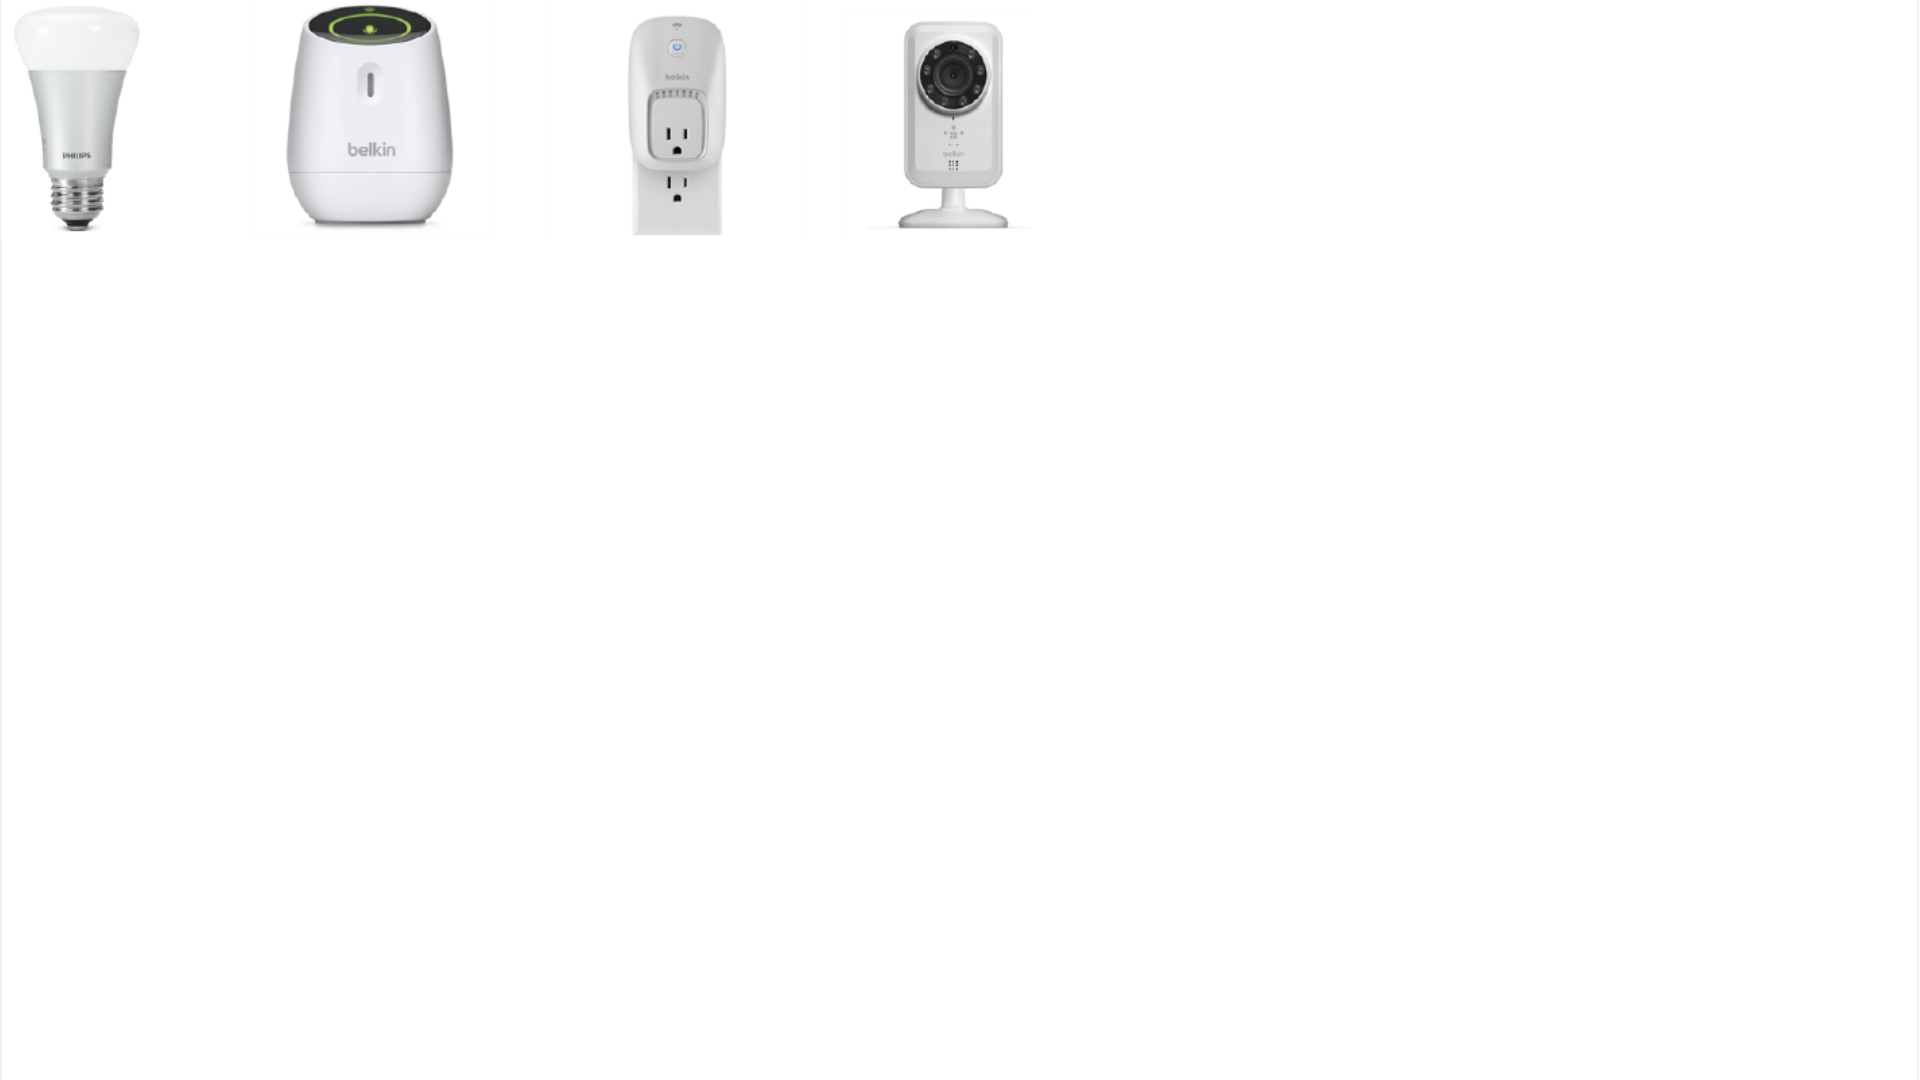
\includegraphics{img/MarketSize.png}
	   \end{center}
	\end{block}
	\begin{block}{New vulnerabilities}
	   \begin{itemize}
	       \item Security is only an afterthought
	       \item Patches rarely get shipped, let alone installed
	   \end{itemize}
	\end{block}	
\end{frame}

\begin{frame}{Practical Relevance (cont.)}
	\begin{block}{Hits close to home (literally)}
	   \begin{center}
		    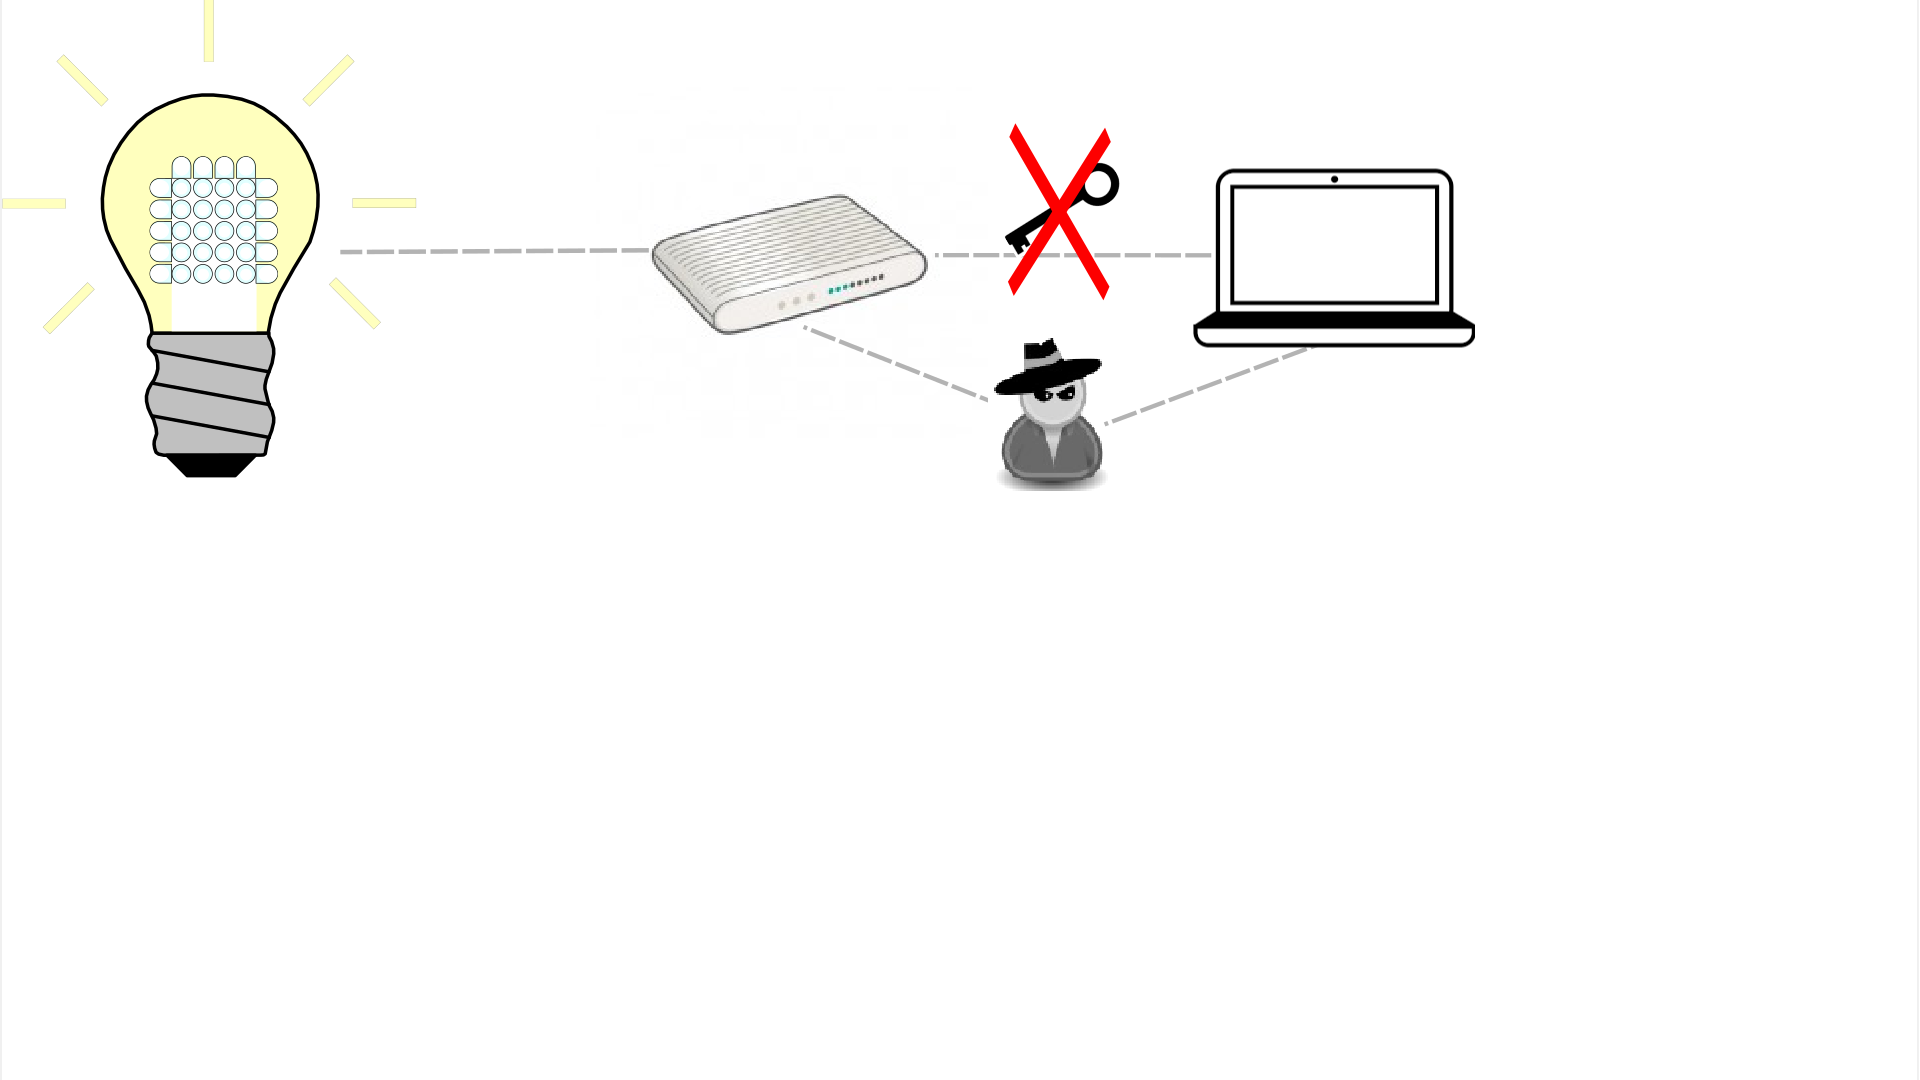
\includegraphics{img/HomeSec.png}
	   \end{center}
	\end{block}
\end{frame}


\begin{frame}{Lights in Particular}
	\begin{center}
        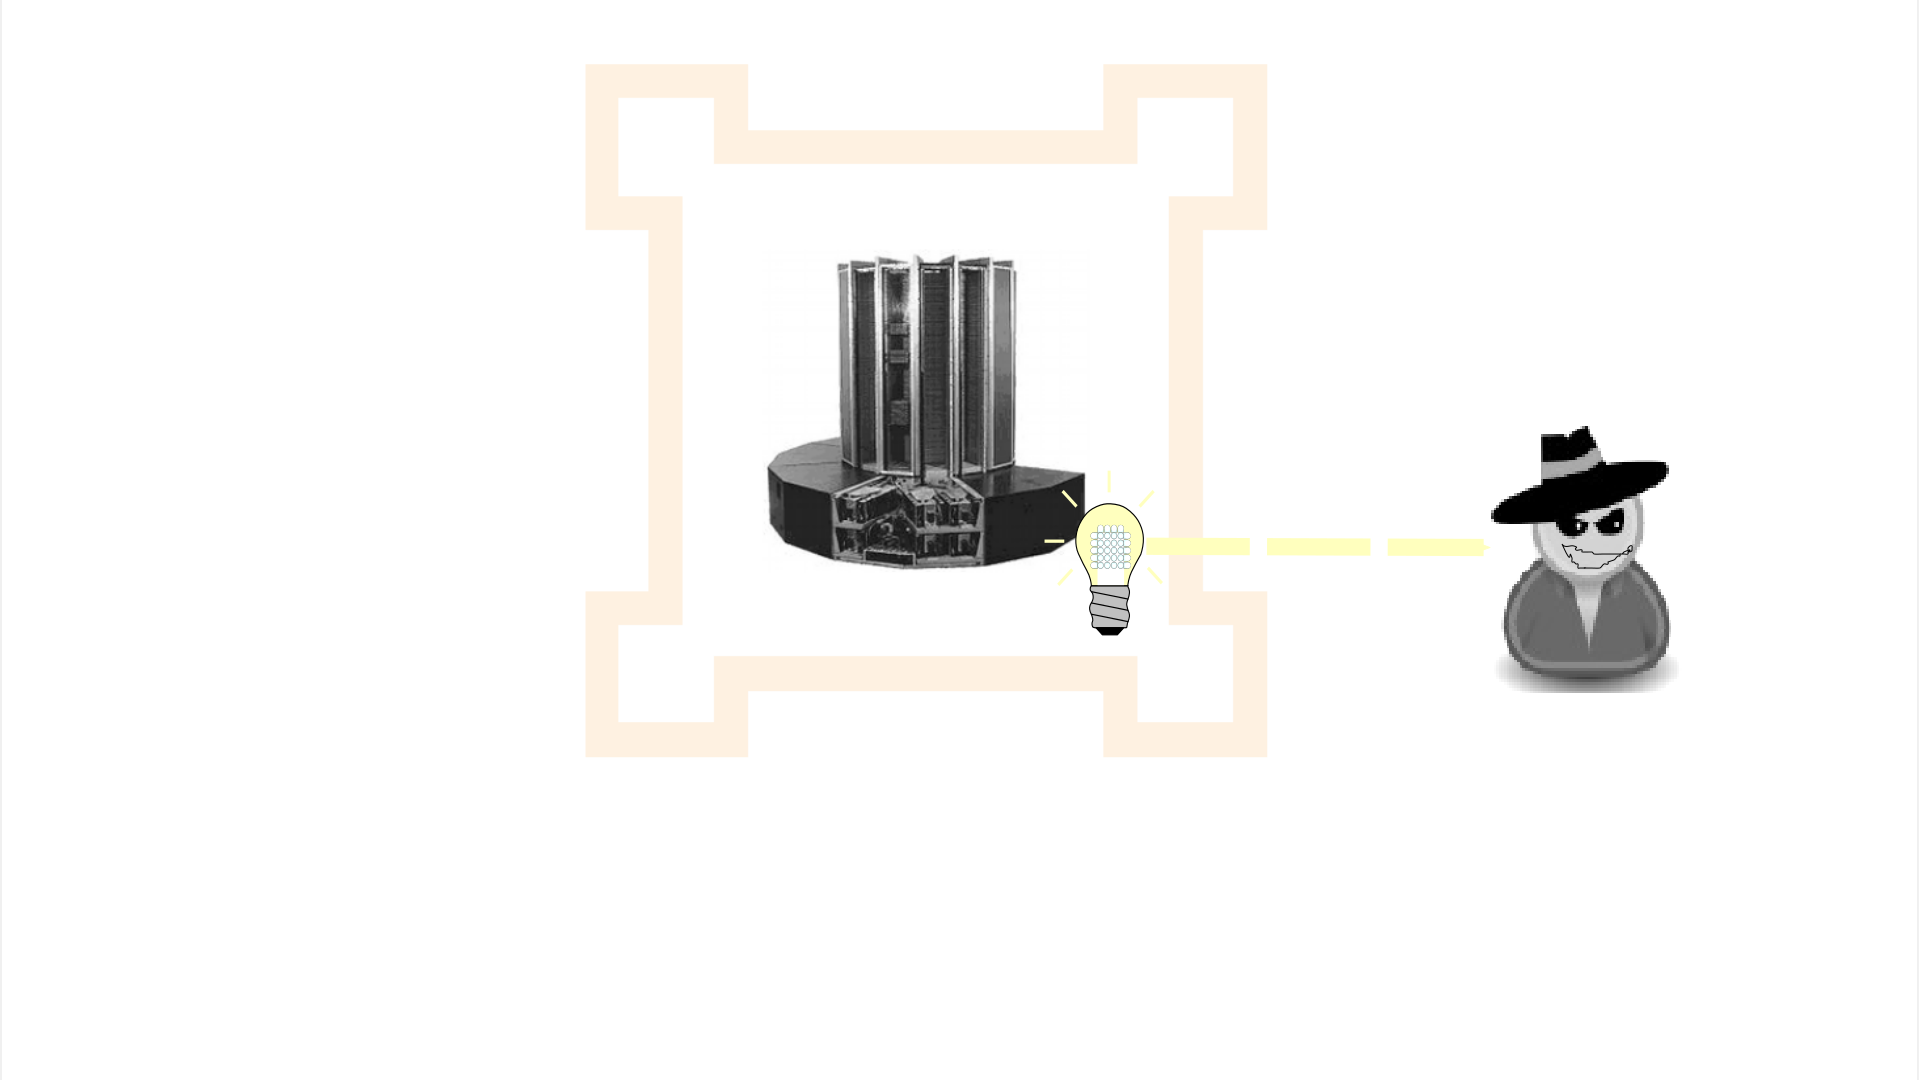
\includegraphics{img/DatacenterIoT.png}
    \end{center}
\end{frame}

%% next PDF bookmark
\subsection{Expected Outcome}

\begin{frame}{Expected Outcome}
	\begin{center}
		\includegraphics{img/Aufbau_1.png}
	\end{center}
\end{frame}

%% to show a last slide similar to the title slide: information for the last page
\title{Questions?}
\subtitle{}
\section{Questions}


%% appendix of 'extra' slides
\appendix

\begin{frame}
\frametitle{Details}
    \begin{block}{Classification of Attacks on IoT Devices}
		We will present a taxonomy of the possible attacks against IoT devices.

		We will then attempt to demonstrate the most interesting kind, namely extending the functionality of a device to make it useful for an attacker:
	\end{block}
	\begin{block}{Our Goals}
		\begin{itemize}
			\item Create a smart light that we can make flicker above $\sim60$ Hz
			\item Even cooler: Abuse API or vulnerabilities of a commercial smart light system
			\item Build a sensor that can capture our high-speed signals
			\item Encode, transmit and decode information over this channel
		\end{itemize}
	\end{block}
\end{frame}

\end{document}

